\documentclass[../main.tex]{subfiles}

\begin{document}

\section{Results}

The torque arm analysis in \textit{Abaqus} uses two distinct loading steps to solve for the stresses generated by the preload and oscillating load conditions.
To properly evaluate the performance of the torque arm under the prescribed loading conditions we combine the stresses of interest after the fact using the built-in post-processing capabilites of the solver.
We can verify the chosen modeling assumptions using the same post-processed data.
Recall, we have assumed that the critical stresses are not located in the bushings, allowing the part to be modeled with discontinous thicknesses.
The other main modeling assumption is that the details of how the loads are applied are not crucial to understanding the critical stress regions. 
To verify these assumptions, we examine the contour plots of Von Mises stresses for both cases shown in figures \ref{baseline_axial_mises}-\ref{baseline_vertical_mises}, noting that the maximums stresses are \textit{not} in the bushing regions, proving that the discontinuous thickness is acceptable.
Next, the net reaction force experienced by the torque arm must match the net force of the applied tractions for preload and oscillating steps.
The ``time'' history of reaction forces during analysis steps is plotted in figures \ref{RF_preload}-\ref{RF_oscillating}, showing agreement with the applied force magnitudes of \(4500\,\unit{\newton}\) and \(900\,\unit{\newton}\) respectively.
The reaction forces of \(-4500\,\unit{\newton}\) and \(-900\,\unit{\newton}\) place the torque arm into static equilibrium during the given analysis steps, confirming our second assumption.

\begin{figure}[H]
    \centering
    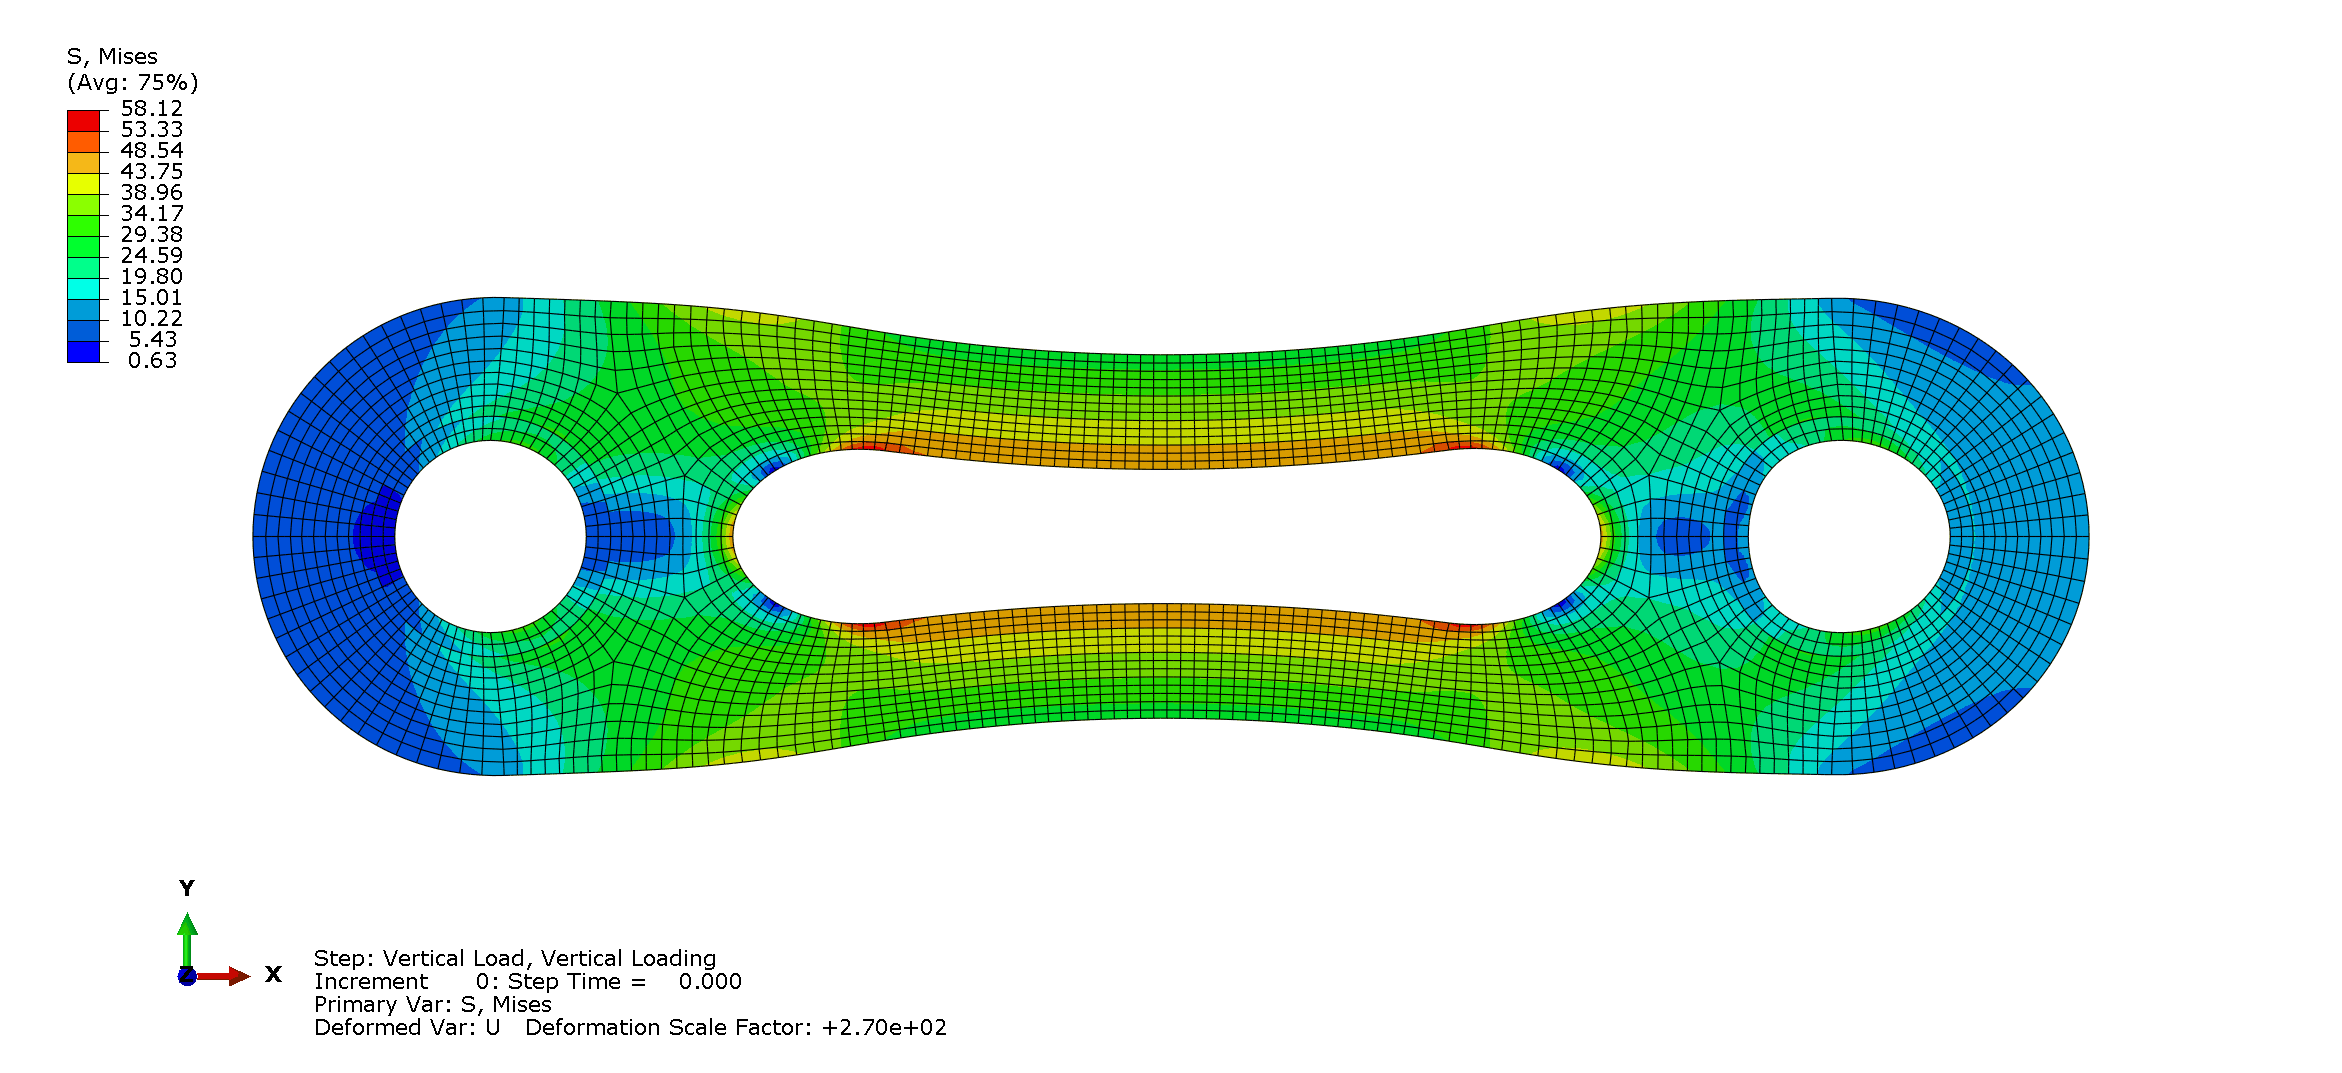
\includegraphics[scale=0.2]{../../images/baseline_axial_mises.png}
    \caption{Contours of Von Mises stress for baseline preload}
    \label{baseline_axial_mises}
\end{figure}

\begin{figure}[H]
    \centering
    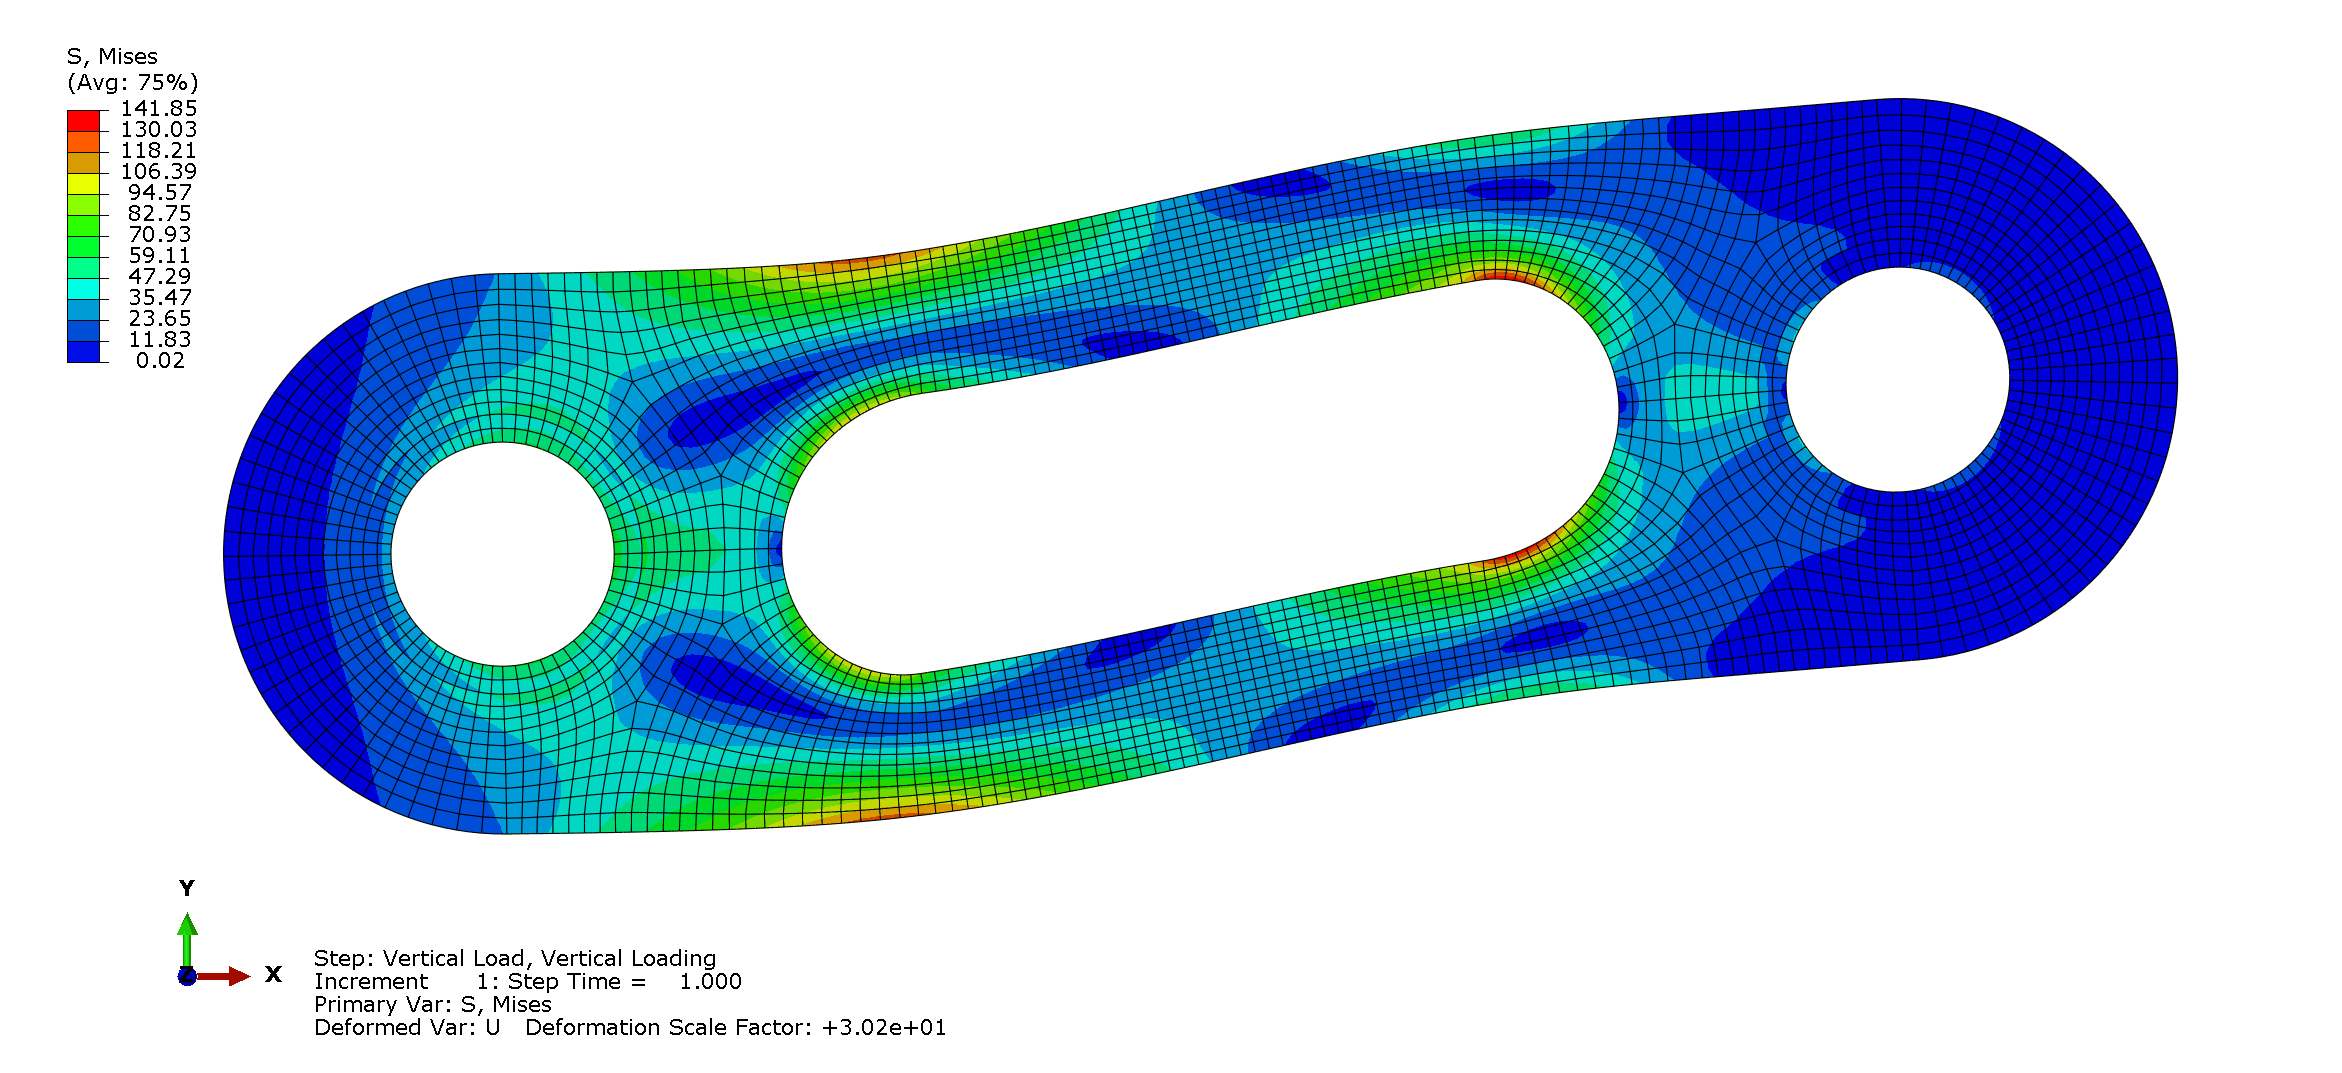
\includegraphics[scale=0.2]{../../images/baseline_vertical_mises.png}
    \caption{Contours of Von Mises stress for baseline oscillating load}
    \label{baseline_vertical_mises}
\end{figure}

\begin{figure}[H]
    \centering
    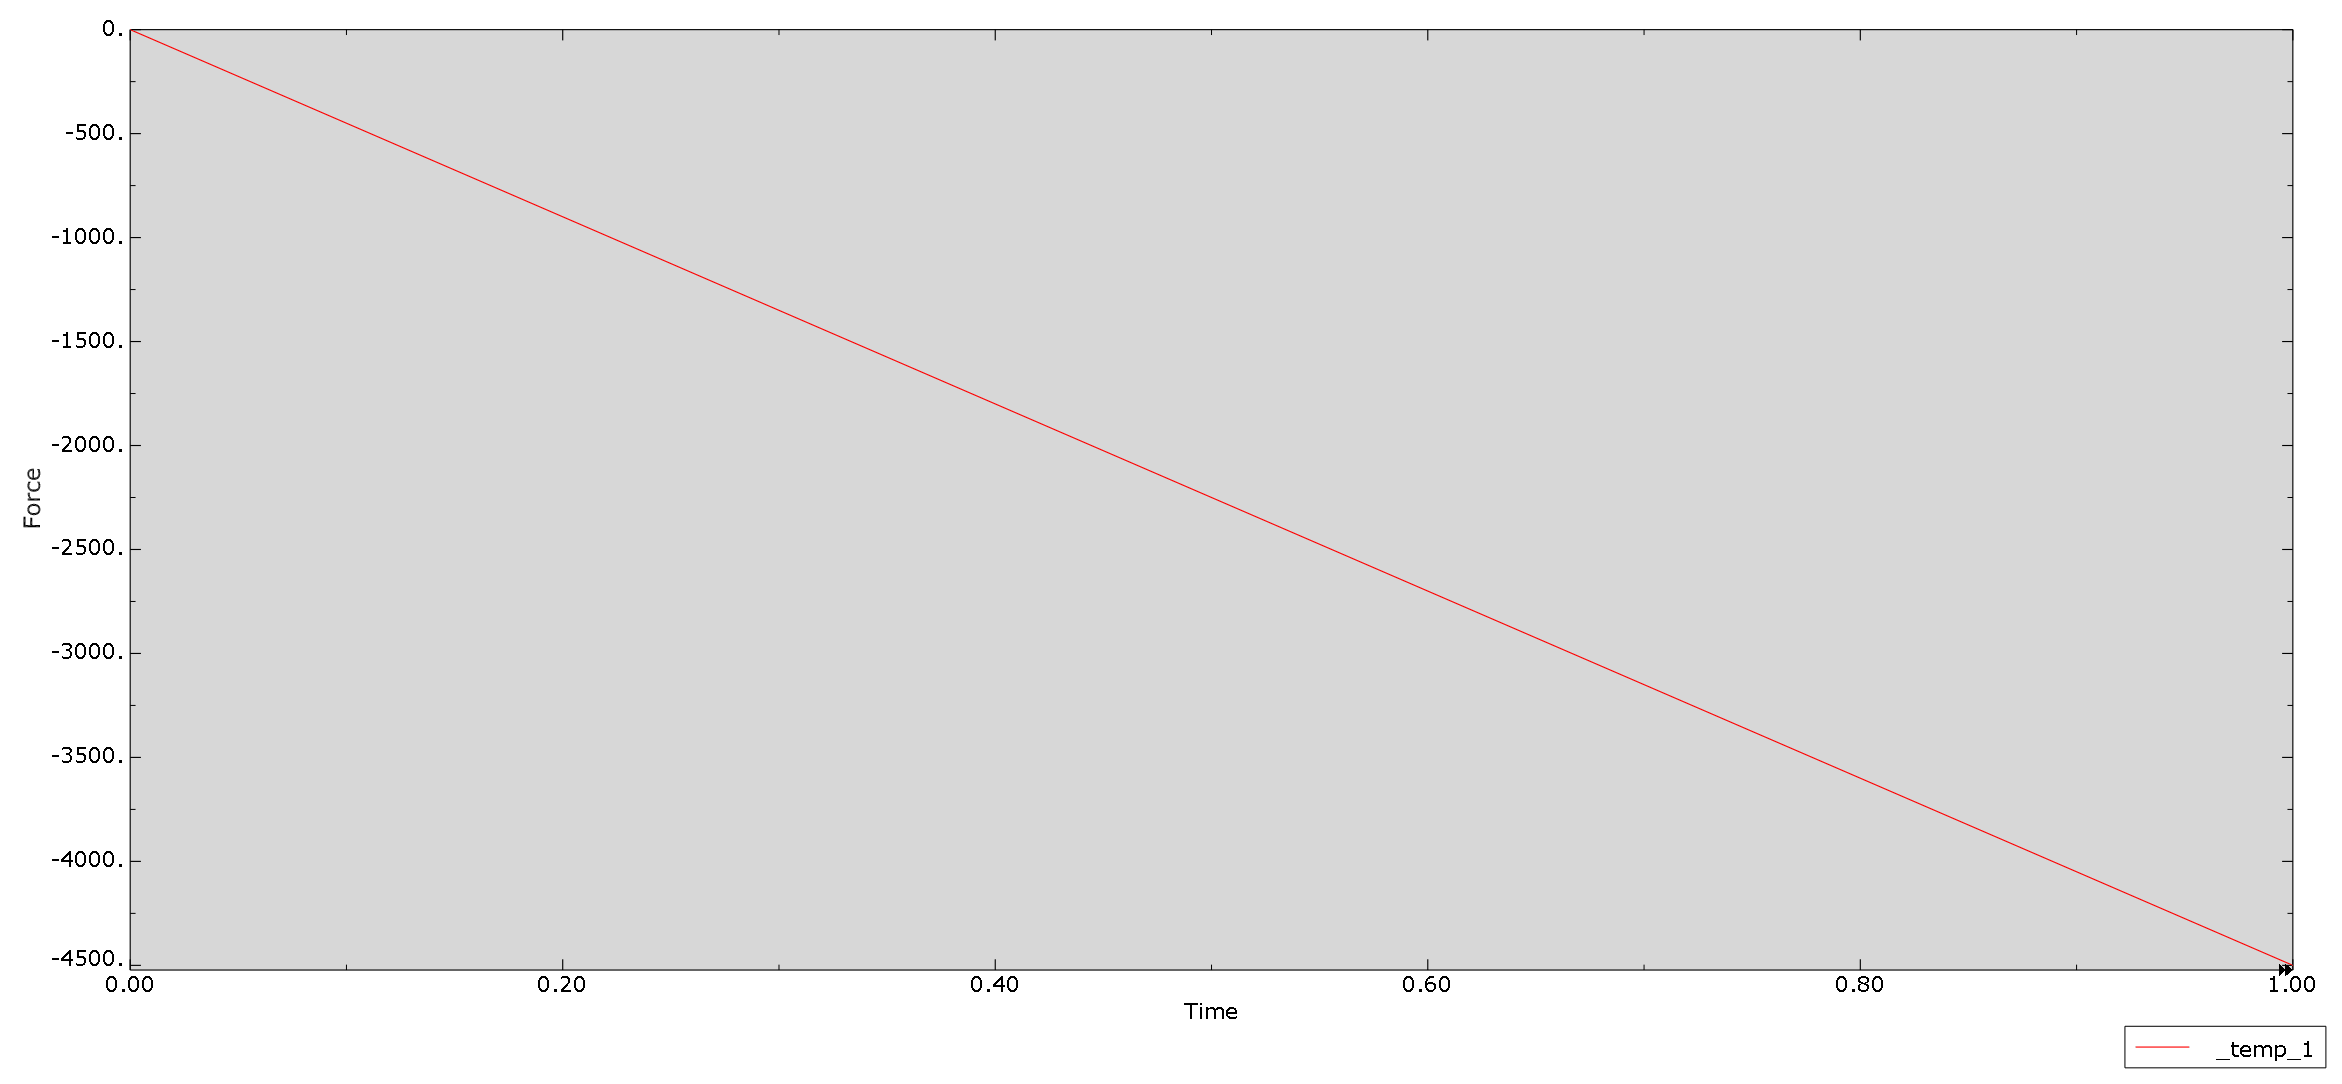
\includegraphics[scale=0.15]{../../images/RF_preload.png}
    \caption{Net reaction force during preload shows agreement with applied load}
    \label{RF_preload}
\end{figure}

\begin{figure}[H]
    \centering
    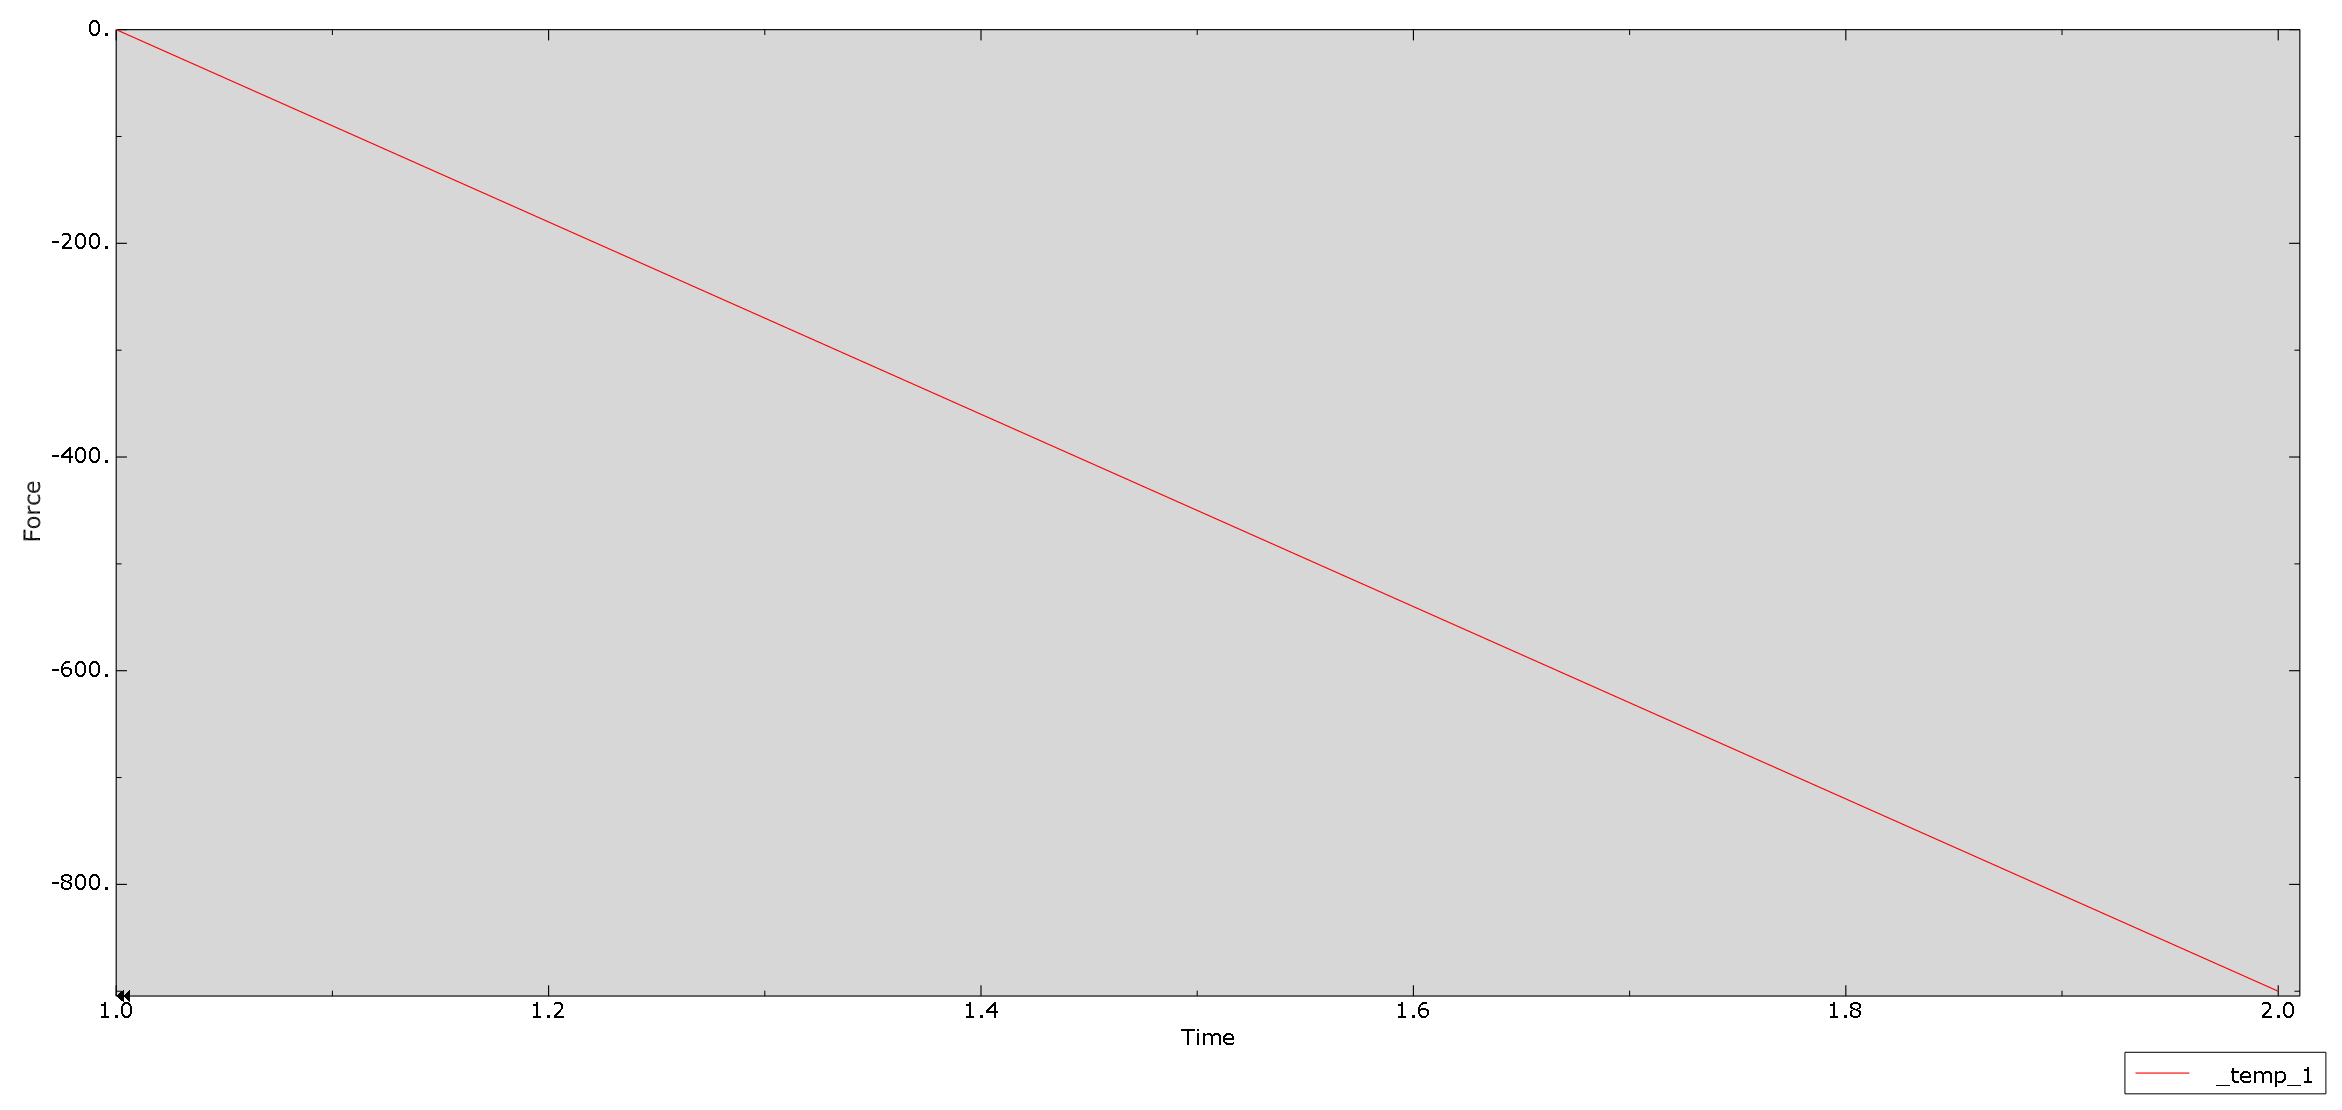
\includegraphics[scale=0.15]{../../images/RF_vertical.png}
    \caption{Net reaction force during oscillating load shows agreement with applied load}
    \label{RF_oscillating}
\end{figure}

Having verified the fundamental assumptions made during analysis, we can now evaluate the failure criteria of the torque arm.
Given a yield strength of \(\sigma_{y}=75\,\unit{\mega\pascal}\) we can check for yield failure by combining the Von Mises stresses from the two loading conditions, shown in figure \ref{baseline_combined_mises}.
Adjusting the scale of the contour plots highlights the regions where the stresses exceed the yield strength, shown in figure \ref{baseline_combined_mises_limited}.
There are several regions which show signs of yielding and failure with Von Mises stress values substantially larger than the yield strength.
The critical region of yielding is located on right side of the torque arm, at the top and bottom of the central gap.

\begin{figure}[H]
    \centering
    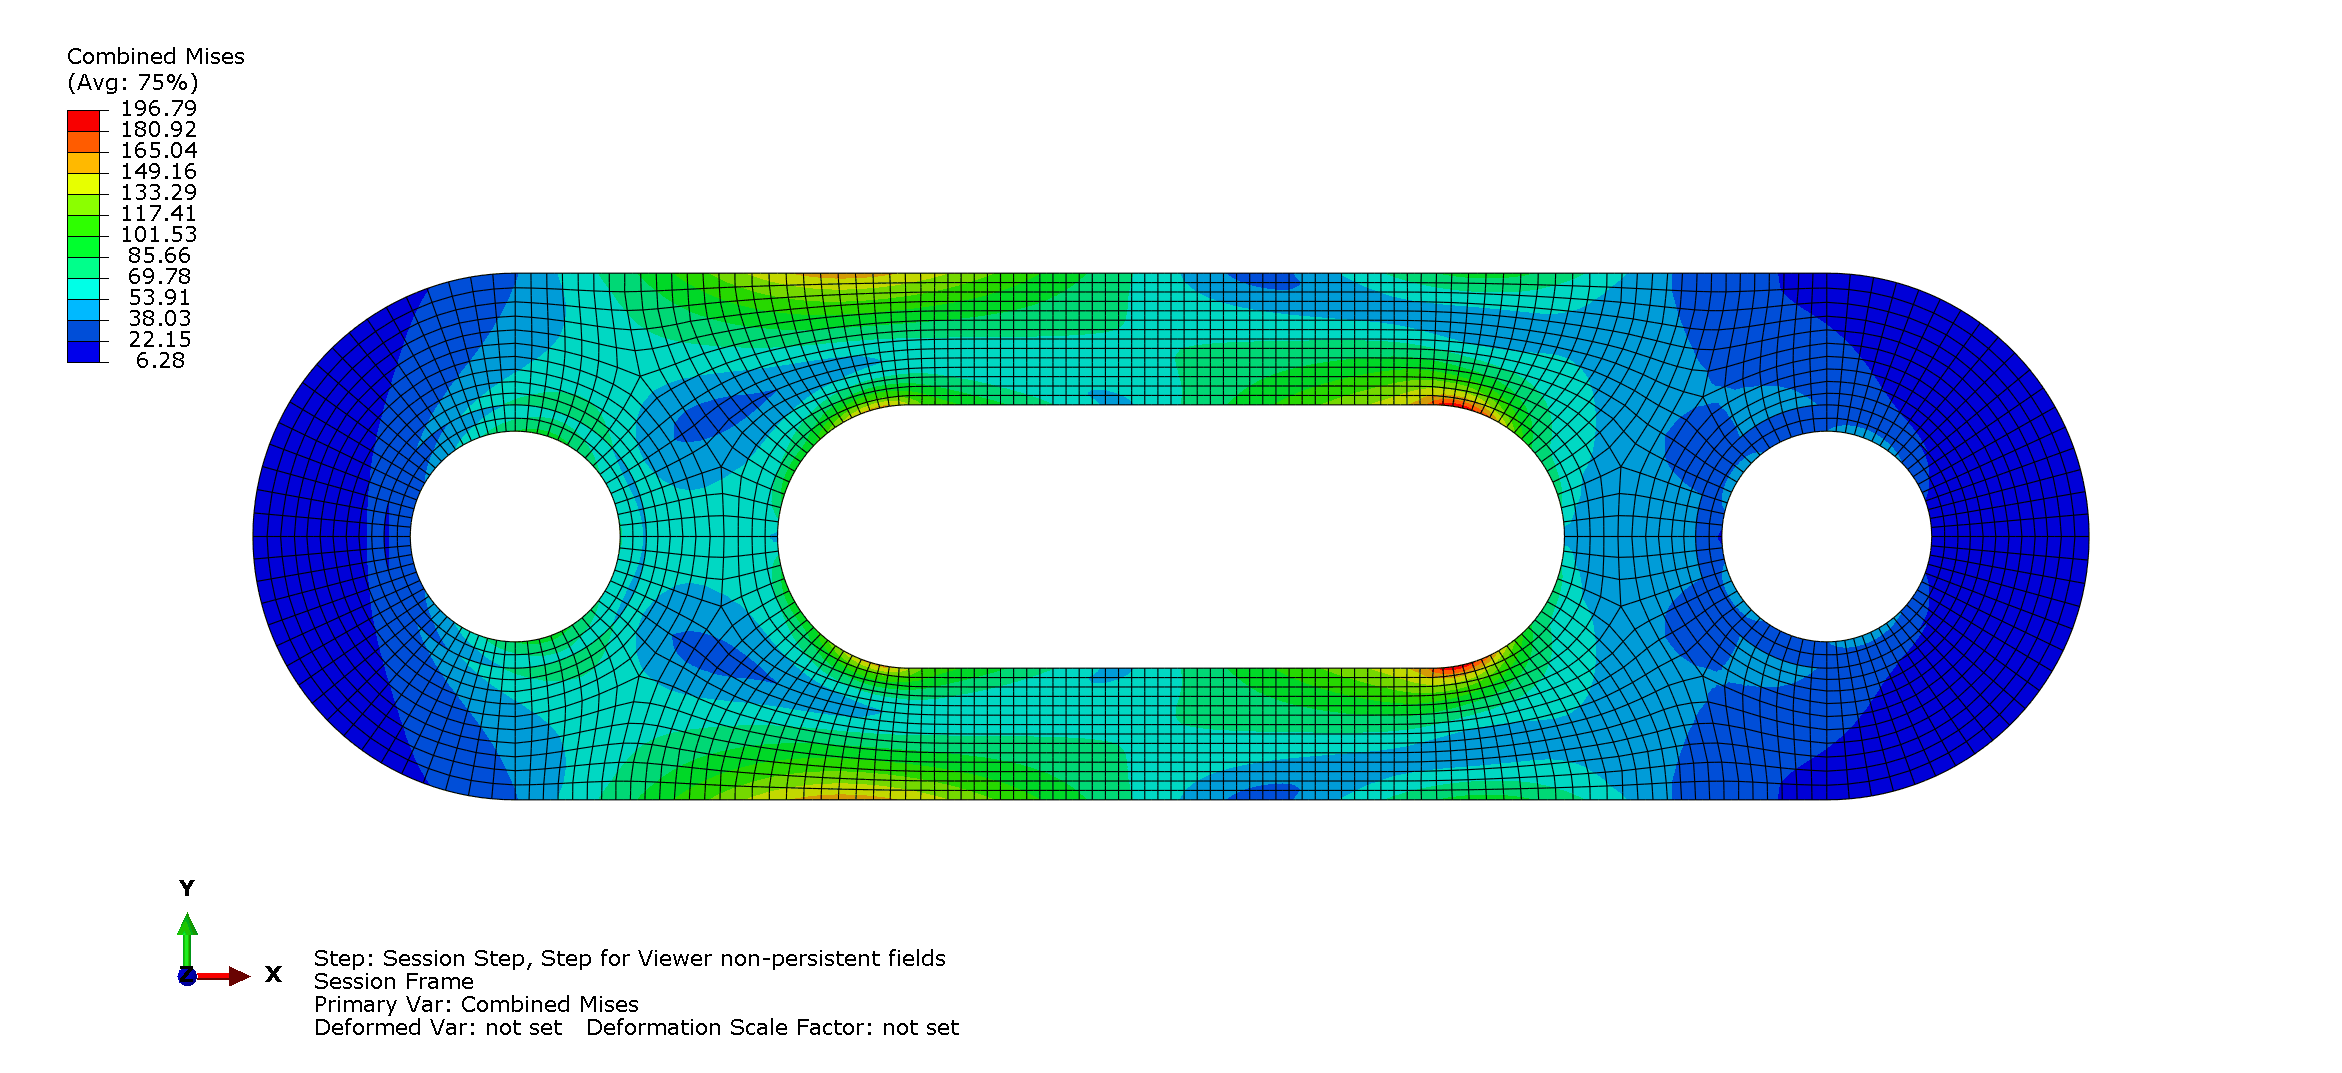
\includegraphics[scale=0.2]{../../images/baseline_combined_mises.png}
    \caption{Contour plot of combined Von Mises stresses}
    \label{baseline_combined_mises}
\end{figure}

\begin{figure}[H]
    \centering
    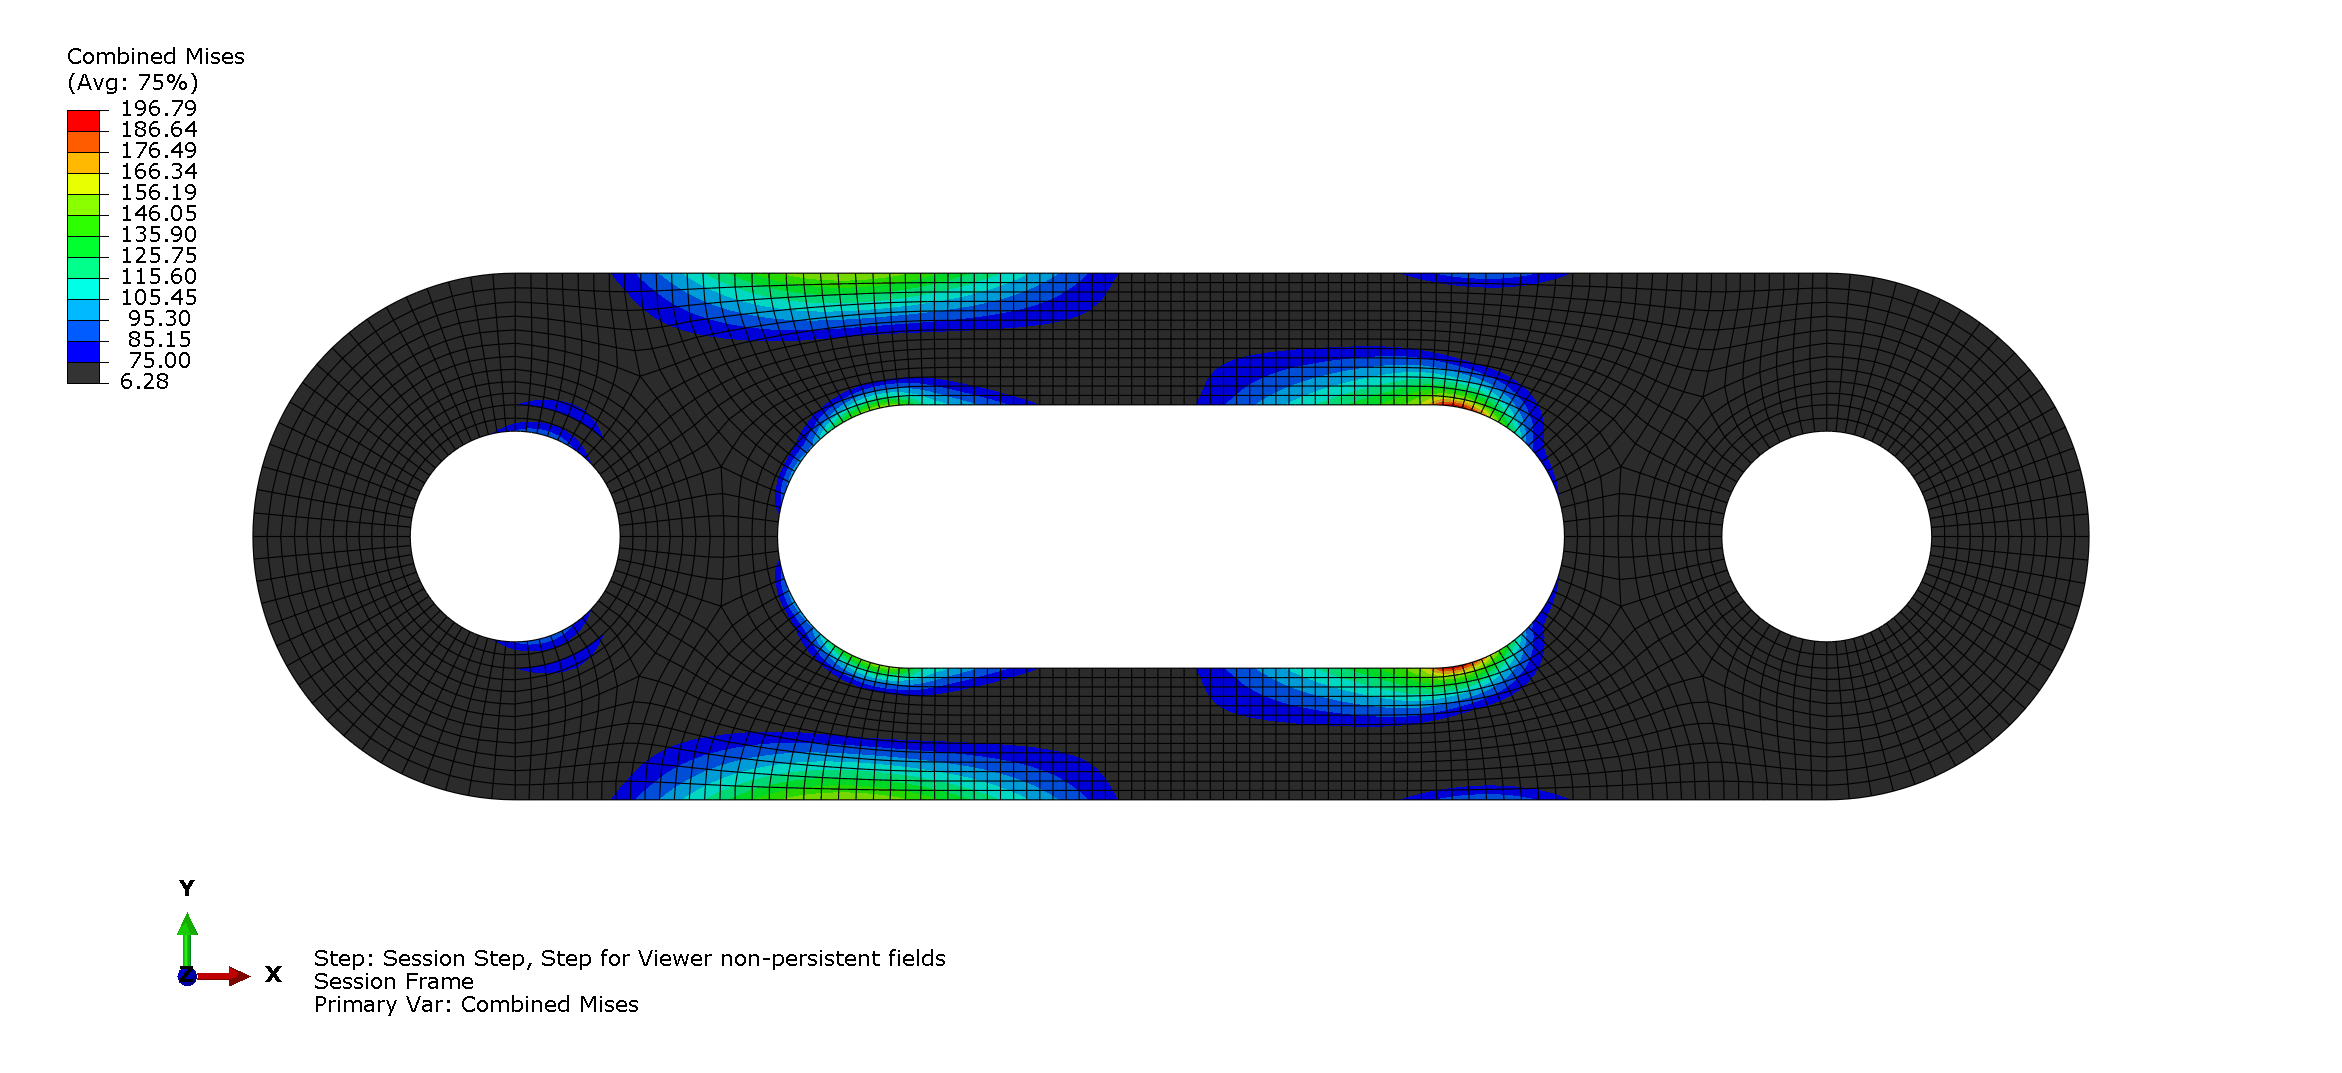
\includegraphics[scale=0.2]{../../images/baseline_combined_mises_limited.png}
    \caption{Contour plot of combined Von Mises stresses with failed regions highlighted}
    \label{baseline_combined_mises_limited}
\end{figure}

To evaluate fatigue failure we utilize the Gerber equation:

\[
    \frac{\sigma_{cyc}}{\sigma_e} + \left({\frac{\sigma_{mean}}{\sigma_y}}\right)^2 = 1
\]

By combining the maximum principal stresses from both loading cases we can assess the potential for failure in fatigue.
The maximum principal stress from preload and the oscillating load are represented by \(\sigma_{mean}\) and \(\sigma_{cyc}\), respectively.
Similar to the yield strength plots, we can generate a contour plot of the value from the Gerber equation to evaluate the entire torque arm and identify all regions that are likely to fail in fatigue at once, shown in figure \ref{baseline_gerber}.
Once again in figure \ref{baseline_gerber_limited}, by limiting the contour scale we can identify all regions that exceed the Gerber limit of 1.
With a peak value of 5.25, the baseline design of the torque arm performs very poorly and requires a dramatic increase in thickness to avoid failure. 
The critical region for fatigue failure is on the right side of the central gap at the bottom. 

\begin{figure}[H]
    \centering
    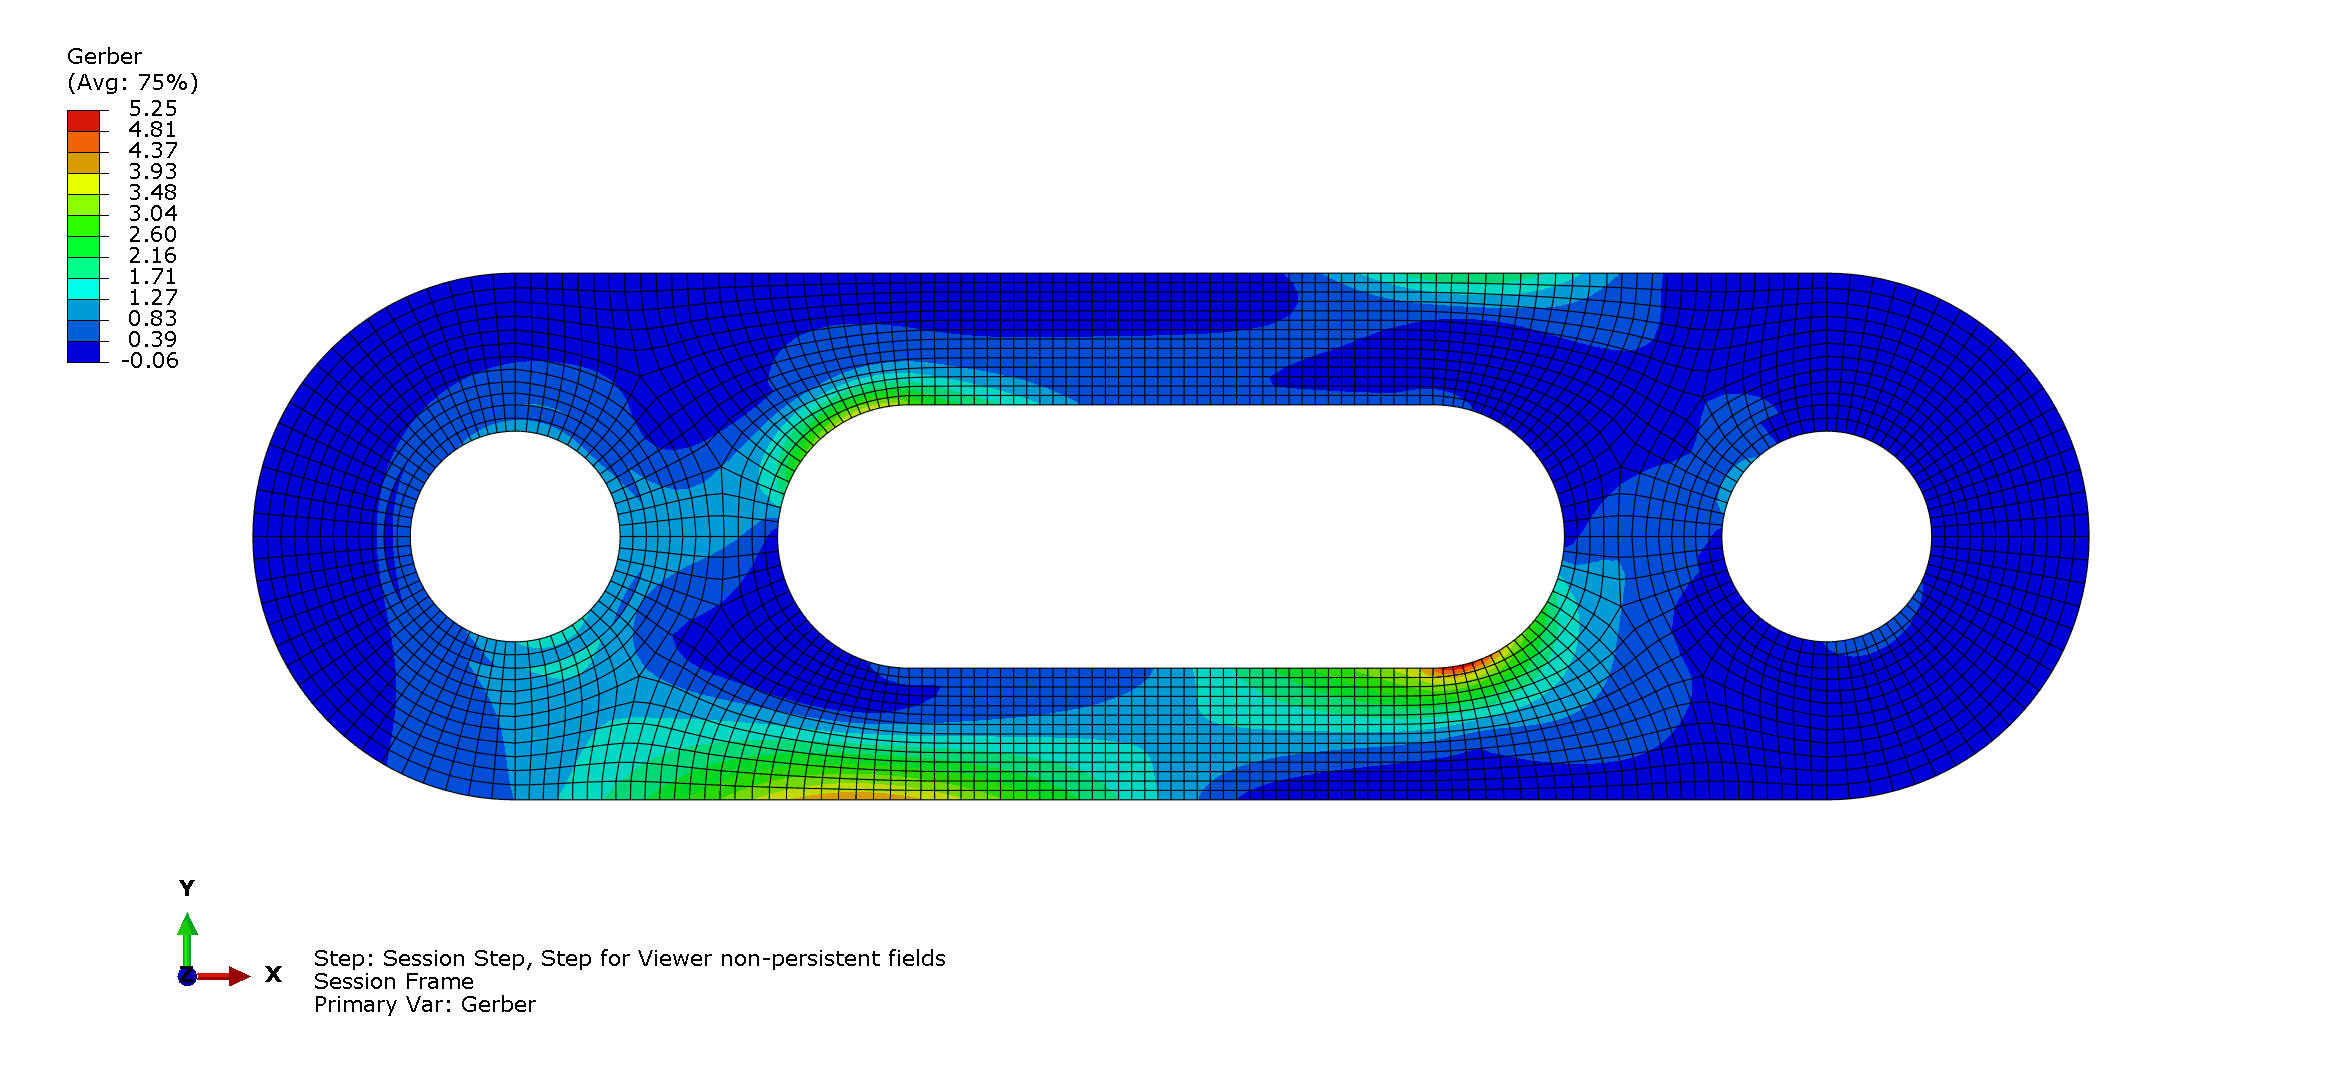
\includegraphics[scale=0.2]{../../images/baseline_gerber.png}
    \caption{Contour plot of Gerber equation values}
    \label{baseline_gerber}
\end{figure}

\begin{figure}[H]
    \centering
    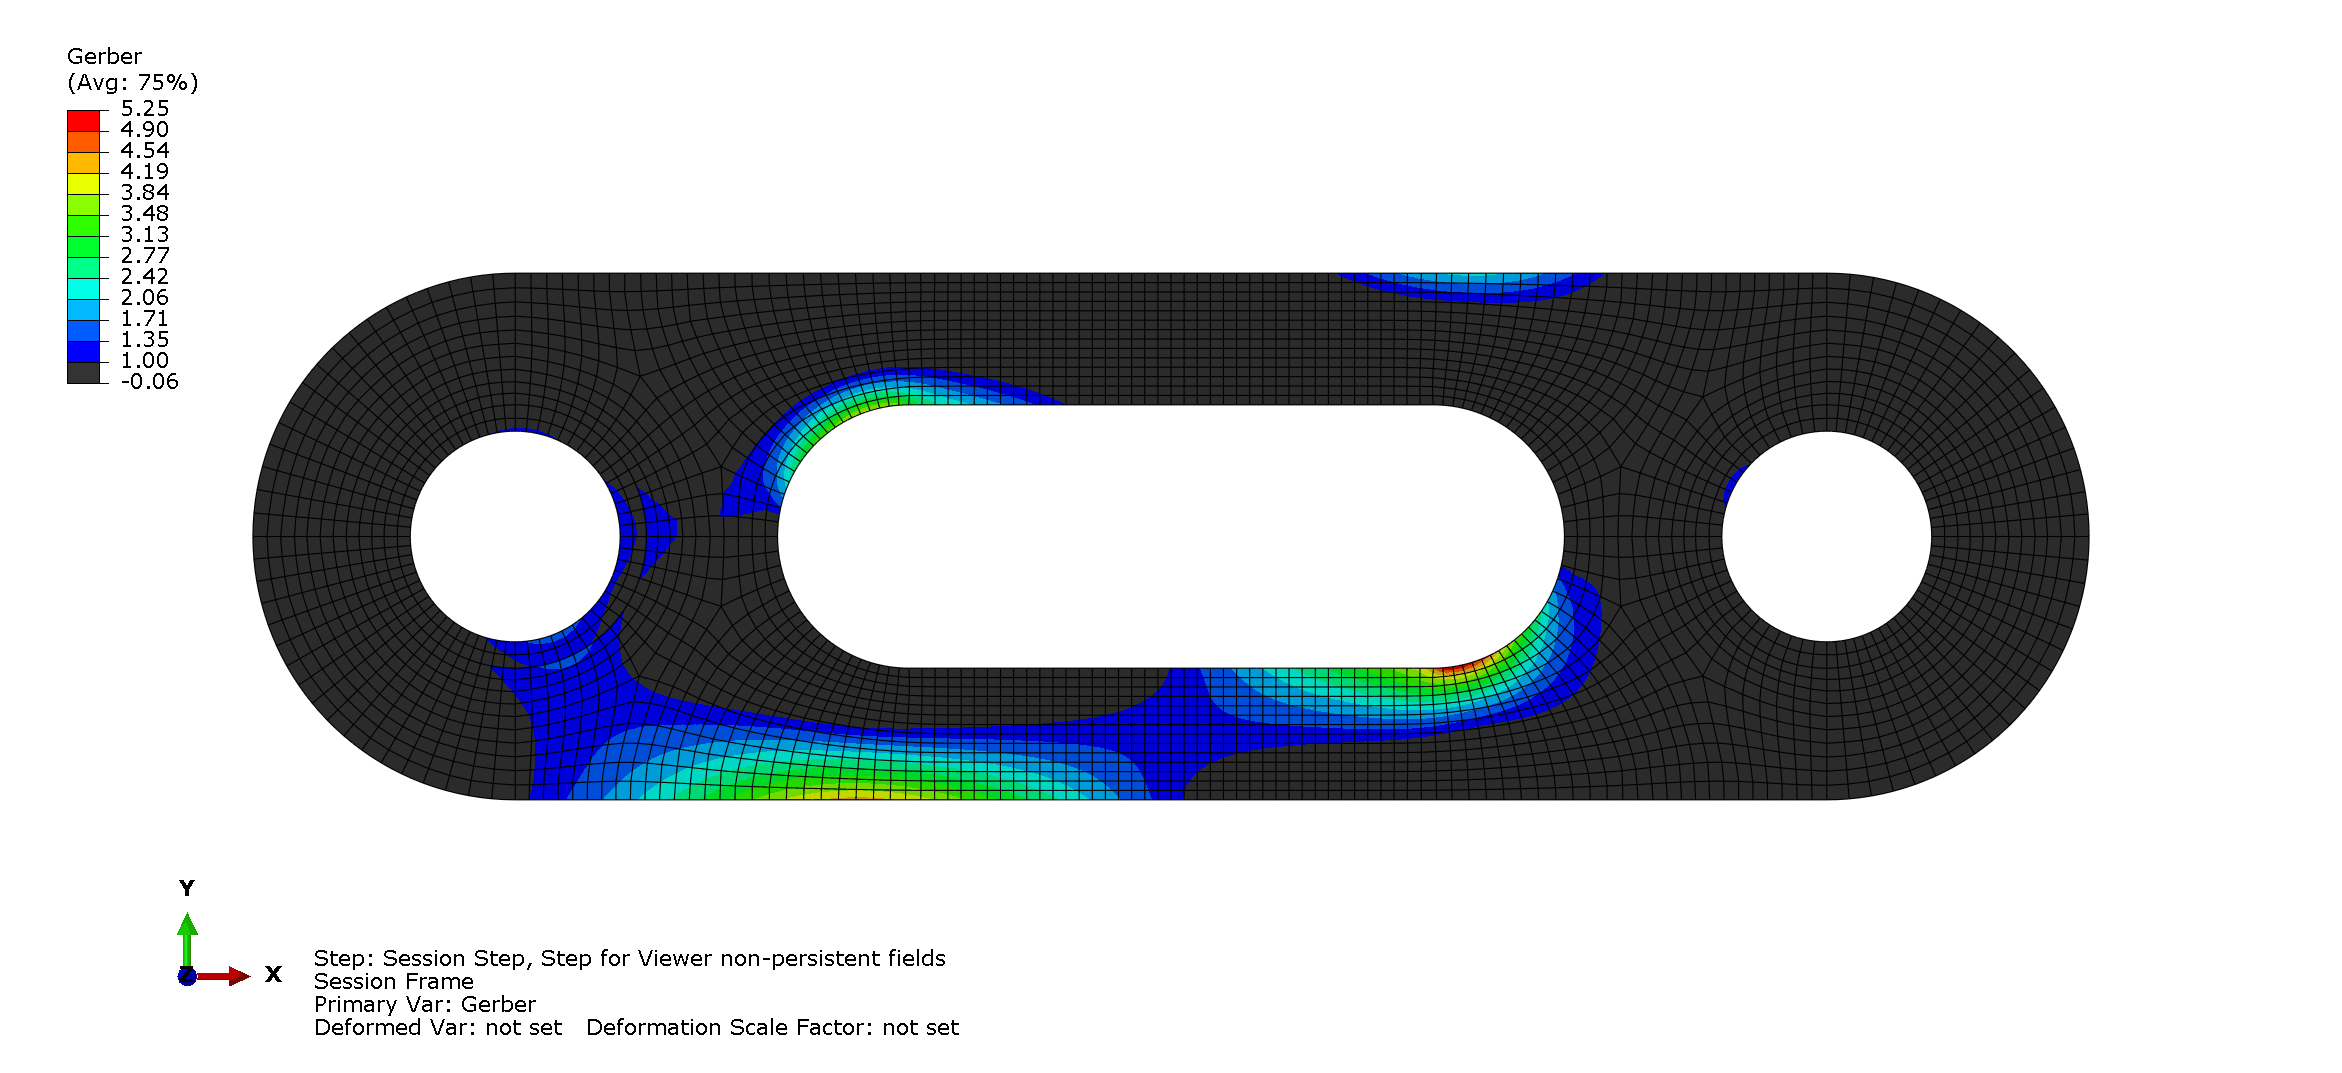
\includegraphics[scale=0.2]{../../images/baseline_gerber_limited.png}
    \caption{Contour plot of Gerber equation values with failed regions highlighted}
    \label{baseline_gerber_limited}
\end{figure}

\end{document}